\subsection{Interfaz de la sección ``Analítica de producciones''}
La interfaz de esta sección está conformada por 6 Cards que contienen información estadística de las producciones que se han realizado y de las piezas de las mismas. 

Las primeras 3 Cards que puede ver el usuario contienen la cantidad de producciones, piezas y canjes que se han realizado hasta la actualidad, además, cada una de estas Cards tiene una comparativa para saber si ha habido un aumento en la creación de los elementos mencionados anteriormente. Como último detalle, las 3 Cards también contienen un botón con la leyenda ``Ver Todo'' ubicado en la esquina superior derecha; el propósito de este botón es mandar al usuario a la sección ``Administración de Producciones'' para que pueda ver la información completa (Ver FIgura 47).

    \begin{figure}[H]
        \begin{center}
            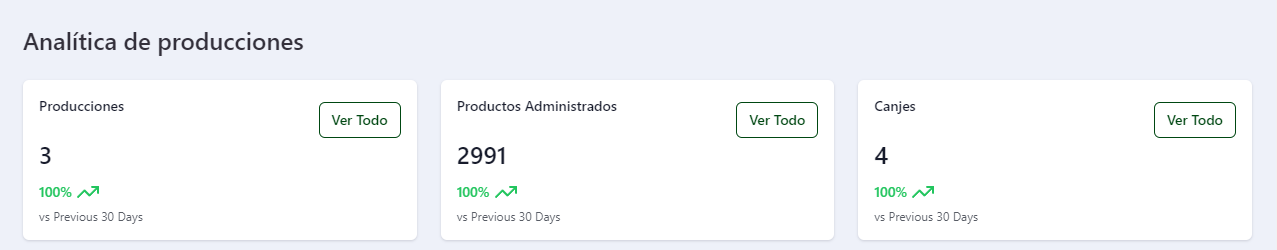
\includegraphics[scale=0.45]{img/actividades/analitica-prod/number-cards.png}
            \caption{Cards con información de producciones, piezas y canjes.}
            \label{fig:number-cards}
        \end{center}
    \end{figure}

Las otras 3 Cards contienen información respecto a los canjes y los estatus de las producciones. Esta información se presenta en forma de gráficas y tablas para facilitar la visualización de la misma. 

Las primeras dos Cards están conformadas por una gráfica de barras y una tabla que muestra 6 registros como máximo, y la información que se muestra aquí son los usuarios y productos más activos (con más canjes). La última Card contiene una gráfica circular que muestra la cantidad de producciones que se encuentran en los diferentes estatus: Aprobado, Pendiente, Cancelado o Finalizado (Ver Figura 48). 

    \begin{figure}[H]
        \begin{center}
            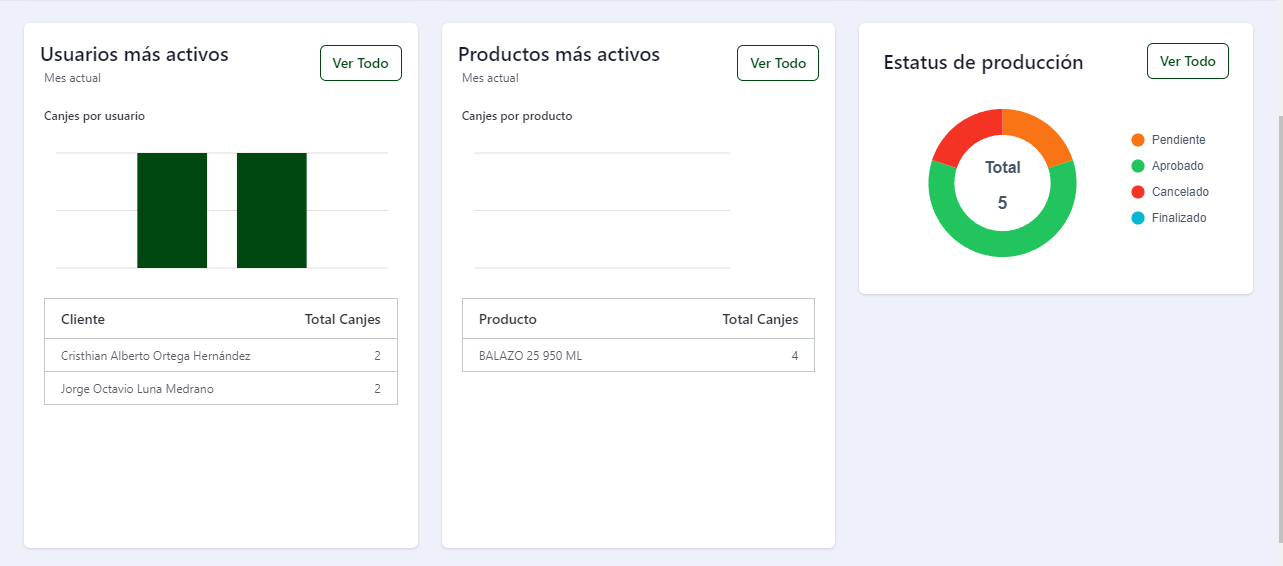
\includegraphics[scale=0.35]{img/actividades/analitica-prod/graficas-cards.png}
            \caption{Cards con gráficas y tablas.}
            \label{fig:graficas-cards}
        \end{center}
    \end{figure}

Todas las Cards contienen un botón con la leyenda ``Ver Todo'', al presionarlo, en las primeras dos Cards, se mostrará un Dialog con una tabla con todos los registros, mientras que la última Card dirigirá al usuario a la sección de ``Administración de Producciones'' (Ver Figura 49).

    \begin{figure}[H]
        \begin{center}
            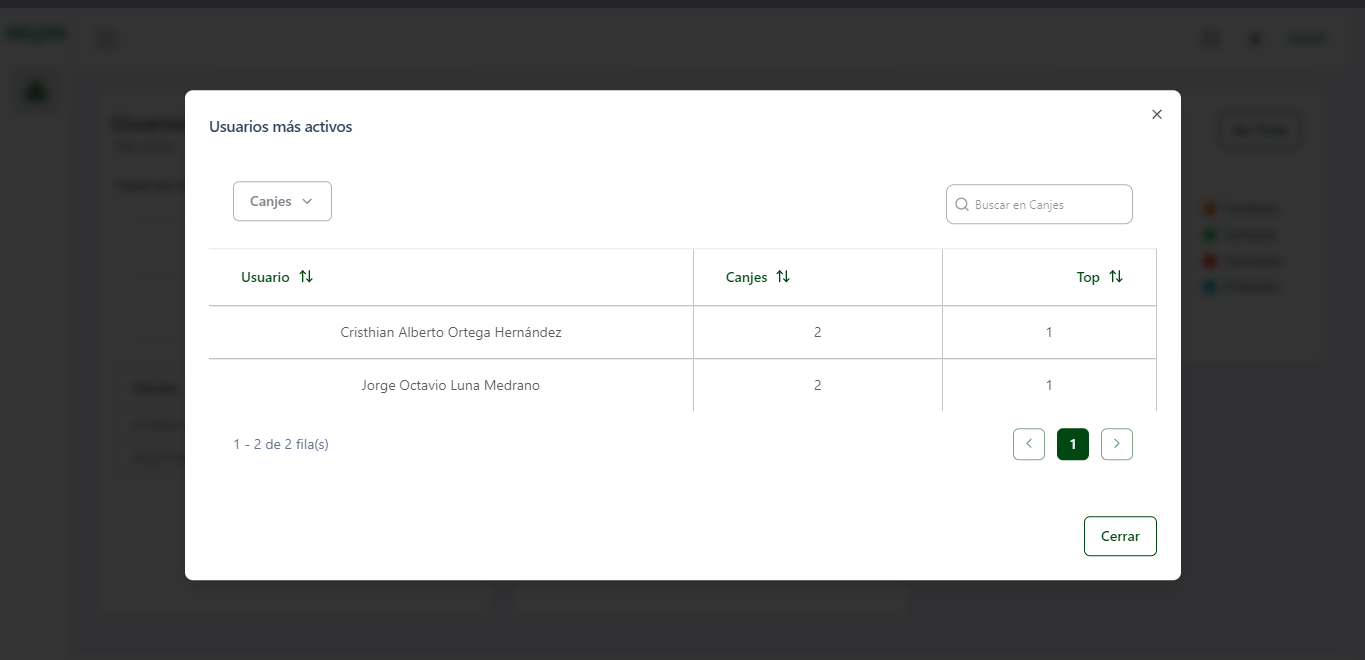
\includegraphics[scale=0.33]{img/actividades/analitica-prod/dialog-tabla.png}
            \caption{Dialgo con tabla para ver todos los registros.}
            \label{fig:dialog-tabla}
        \end{center}
    \end{figure}